% Tento soubor nahraďte vlastním souborem s obsahem práce.
%=========================================================================
% Autoři: Michal Bidlo, Bohuslav Křena, Jaroslav Dytrych, Petr Veigend a Adam Herout 2019


\chapter{Úvod}
\label{uvod}

\chapter{Teorie}
\label{teorie}
Cílem této kapitoly je seznámit čtenáře s koncepty nutnými pro pochopení 

\section{Voxel}
Jak uvádí kniha \cite{gfx_principles_practice}, voxel, nebo-li \textbf{vo}lume \textbf{el}ement, reprezentuje hodnotu na pravidelné mřížce ve 3D prostoru (obrázek \ref{fig:3d_grid}). Díky tomu, že je prostor rozdělen mřížkou pravidelně, lze voxel definovat pomocí třísložkového vektoru (rovnice \ref{eq:voxel_coords}). Pro účely vykreslování jsou voxelům přiřazovány další vlastnosti, jako například barva nebo materiál.

\begin{equation} \label{eq:voxel_coords}
\begin{gathered}
\vec{pozice_{voxel}} \in \mathbb{Z}_3
\end{gathered}
\end{equation}

\begin{figure}[H]
    \centering
    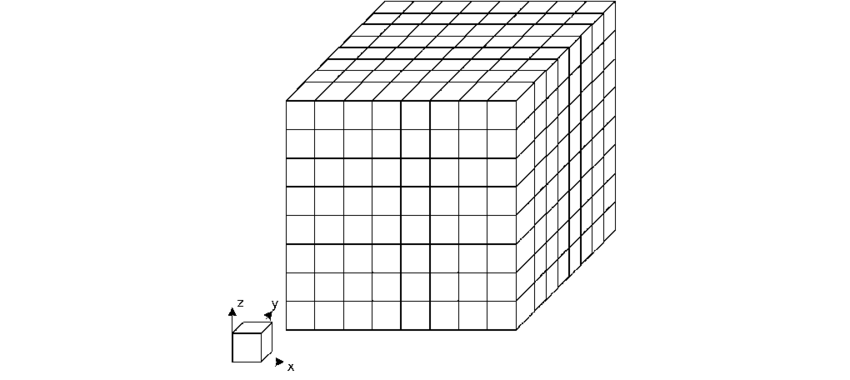
\includegraphics[scale=0.5]{obrazky-figures/3d_grid.png}
    \caption{3D mřížka. \textbf{Zdroj: }\url{https://www.researchgate.net/figure/The-three-dimensional-3D-Cartesian-grid-applied-on-the-simulation-domain-The-latter_fig1_234106571}}
    \label{fig:3d_grid}
\end{figure}

Voxely jsou často využívány v medicíně \cite{medical_vox}, například pro výstupy magnetické resonance (obrázek \ref{fig:mri_vox}).

\begin{figure}[H]
    \centering
    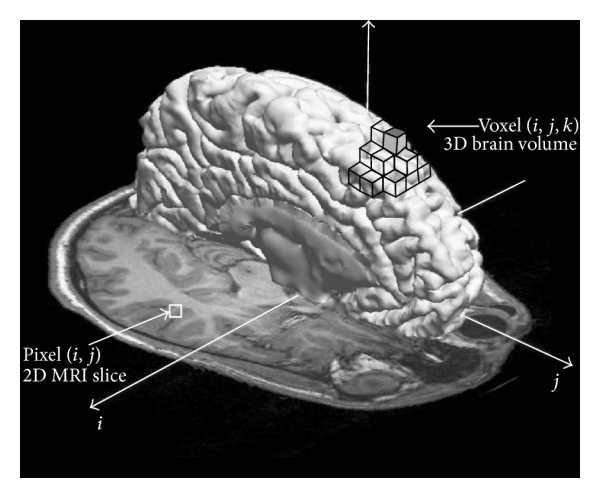
\includegraphics[scale=1]{obrazky-figures/voxel_mri.png}
    \caption{Zobrazení výsledku magnetické resonance pomocí voxelů. \textbf{Zdroj: \cite{mri}}}
    \label{fig:mri_vox}
\end{figure}

Dalším častým využitím je modelování terénu; Voxely přináší možnost reprezentovat převisy, čímž je terén značně realističtější, než při často používaných výškových mapách. Pravděpodobně nejznámější software používající voxely pro terén je Minecraft (obrázek \ref{fig:minecraft}). Za zmínku stojí také hra Teardown (2020)\footnote{\url{https://www.teardowngame.com/}}, kde je celý herní svět vytvořen pomocí voxelů a umožňuje téměř neomezenou destrukci.

\begin{figure}[H]
    \centering
    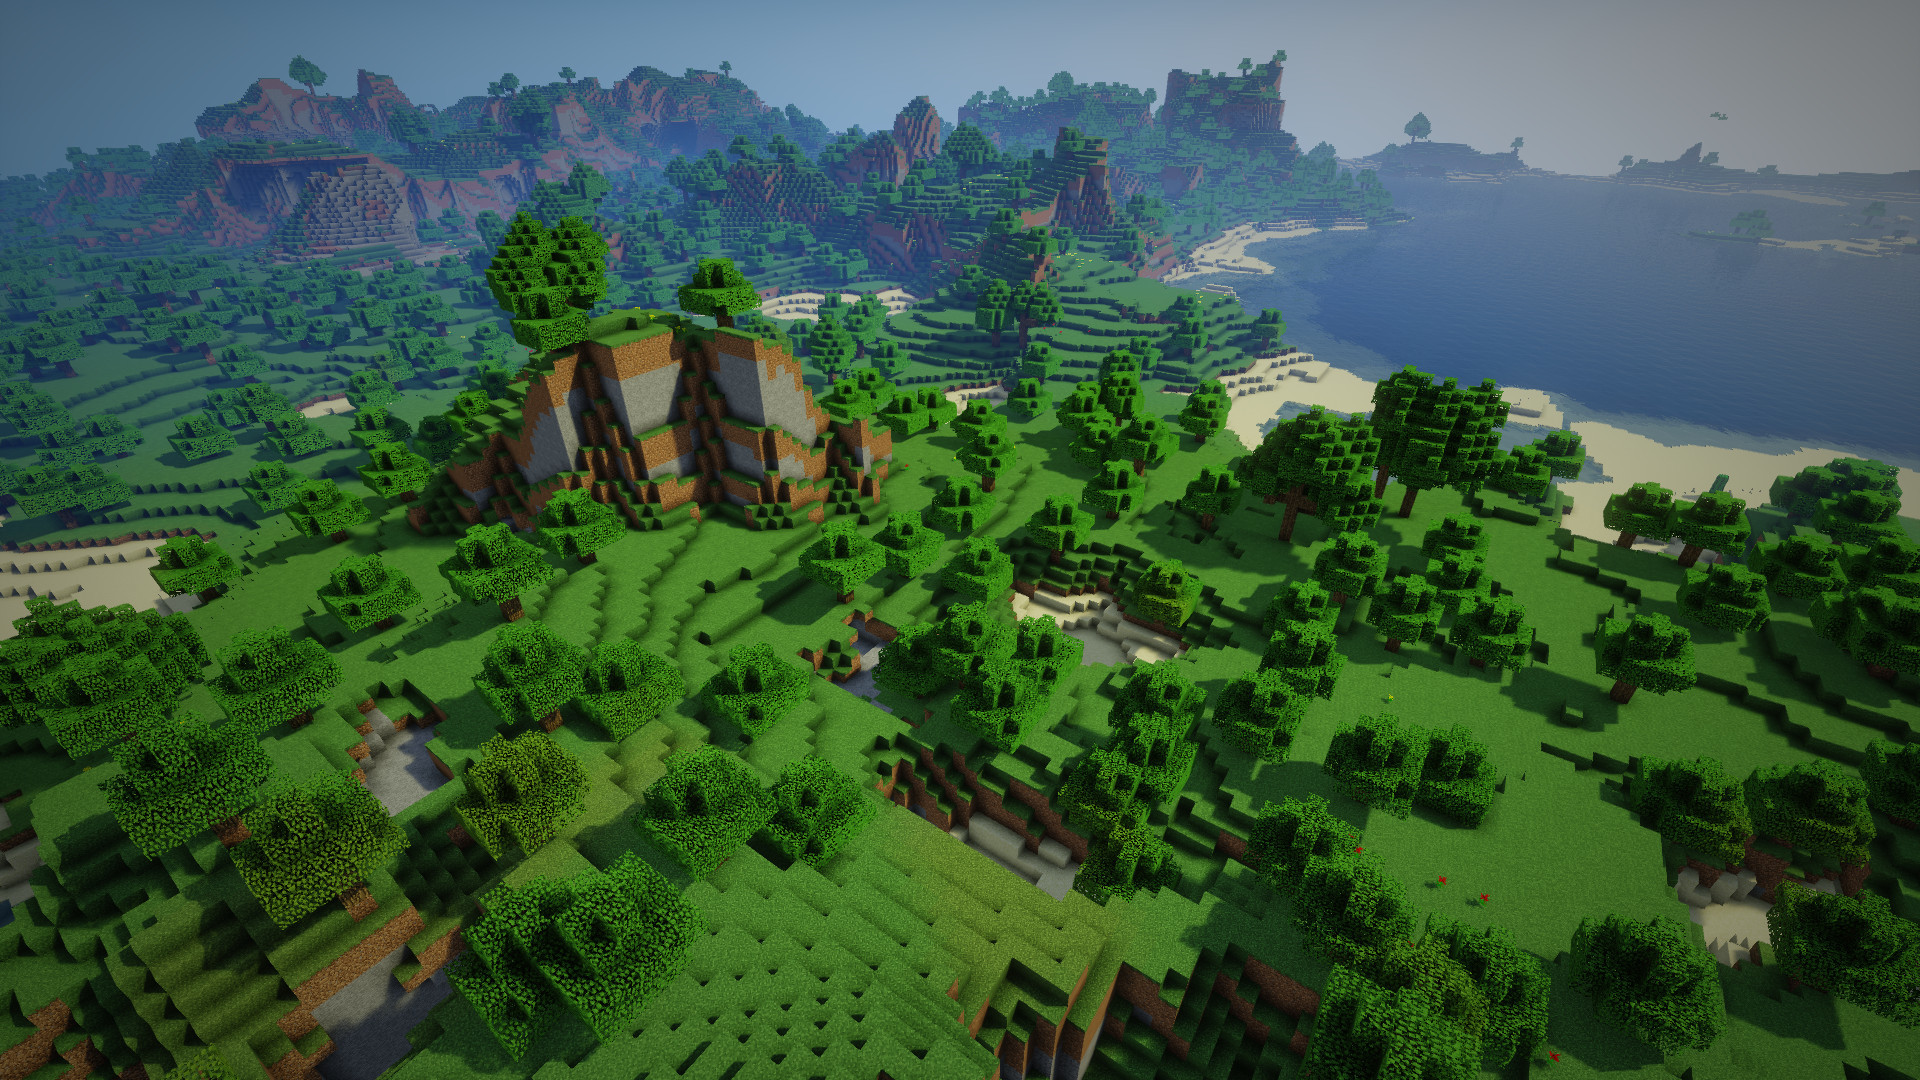
\includegraphics[scale=0.2]{obrazky-figures/minecraft.jpg}
    \caption{Minecraft. \textbf{Zdroj: \url{https://forums-cdn.spongepowered.org/uploads/default/original/2X/8/83abd20efc6cf5104c2f8c5459808bcd1addef7a.jpg}}}
    \label{fig:minecraft}
\end{figure}

\subsection{Vykreslování voxelových modelů}

\subsubsection{Rasterizace}
\subsubsection{Ray casting}

\subsection{Používané formáty}

fotorealisticke zobrazovani

 - global illumination

 - Ray casting
 
 - materialy a tak

voxely 

 - co to je
 
 - jak jsou modely
 
 - zobrazovaci metody
 
 - formaty

Akceleracni struktury

 - zadne
 
 - grid
 
 - octree/svo
 
GPU vulkan

 - co je akcelerace na gpu

 - pipelines

\chapter{Návrh řešení}
\label{navrh}
oduvodneni SVO

popis ray casting algoritmu

popis light field probes

\chapter{Implementace}
\label{implementace}
nacitani a tvorba SVO


\chapter{Testování a vyhodnocení}
\label{testovani}
udelat graf podle poctu voxelu nebo neco

pametova narocnost

\chapter{Další práce}
\label{dalsi_prace}
co je potreba nacit/dodelat


\chapter{Závěr}
\label{zaver}




%===============================================================================
